\documentclass[dvipdfmx,autodetect-engine,titlepage]{jsarticle}
\usepackage[dvipdfm]{graphicx}
\usepackage{ascmac}
\usepackage{fancybox}
\usepackage{listings}
\usepackage{plistings}
\usepackage{itembkbx}
\usepackage{amsmath}
\usepackage{amssymb}
\usepackage{amsfonts}
\usepackage{svg}
\usepackage{url}
\usepackage{graphics}
\usepackage{listings,jvlisting}

\lstset{
  basicstyle={\ttfamily},
  identifierstyle={\small},
  commentstyle={\smallitshape},
  keywordstyle={\small\bfseries},
  ndkeywordstyle={\small},
  stringstyle={\small\ttfamily},
  frame={tb},
  breaklines=true,
  columns=[l]{fullflexible},
  numbers=left,
  xrightmargin=0zw,
  xleftmargin=3zw,
  numberstyle={\scriptsize},
  stepnumber=1,
  numbersep=1zw,
  lineskip=-0.5ex
}

\textheight=23cm
\renewcommand{\figurename}{図}
\renewcommand{\tablename}{表}
\newenvironment{code}
{\vspace{0.5zw}\VerbatimEnvironment  
\begin{screen} 
\baselineskip=1.0\normalbaselineskip
 \begin{Verbatim}}
{\end{Verbatim}
\baselineskip=\normalbaselineskip
 \end{screen}\vspace{0.5zw}} 

\title{情報理工学部 SNコース 3回\\
ワイヤレス通信システム\\
8th Week 演習問題}
\author{2600200443-6\\Yamashita Kyohei\\山下 恭平}
\date{Jun 20 2022}

\begin{document}

\maketitle

\section{78°であることの検証}

\begin{align*}
  D(\theta) = \frac{\cos(\frac{\pi}{2}\cos\theta)}{\sin\theta}
\end{align*}

アンテナの指向性係数が最大となるのは\begin{math}\theta = 90°\end{math}のとき
の1なので、半値角\begin{math}78°\end{math}より、\begin{math}\theta = 90°\pm39°\end{math}
の時に、指向性係数が\begin{math}\frac{1}{\sqrt{2}}\end{math}となれば良い。\\
これをMatlabを用いて検証したものが以下の図と、ソースコードである。

\begin{lstlisting}[caption=hoge,label=fuga]

  theta1 = deg2rad(90 - 78/2);

  theta2 = deg2rad(90 + 78/2);
  
  D1 = cos((pi/2).*cos(theta1))./sin(theta1);
  
  D2 = cos((pi/2).*cos(theta2))./sin(theta2);
  
  y = 1/2^(1/2);
  
  disp(y)
  
  disp(D1)
  
  disp(D2)
 \end{lstlisting}

 \begin{figure}[h]
  \centering
  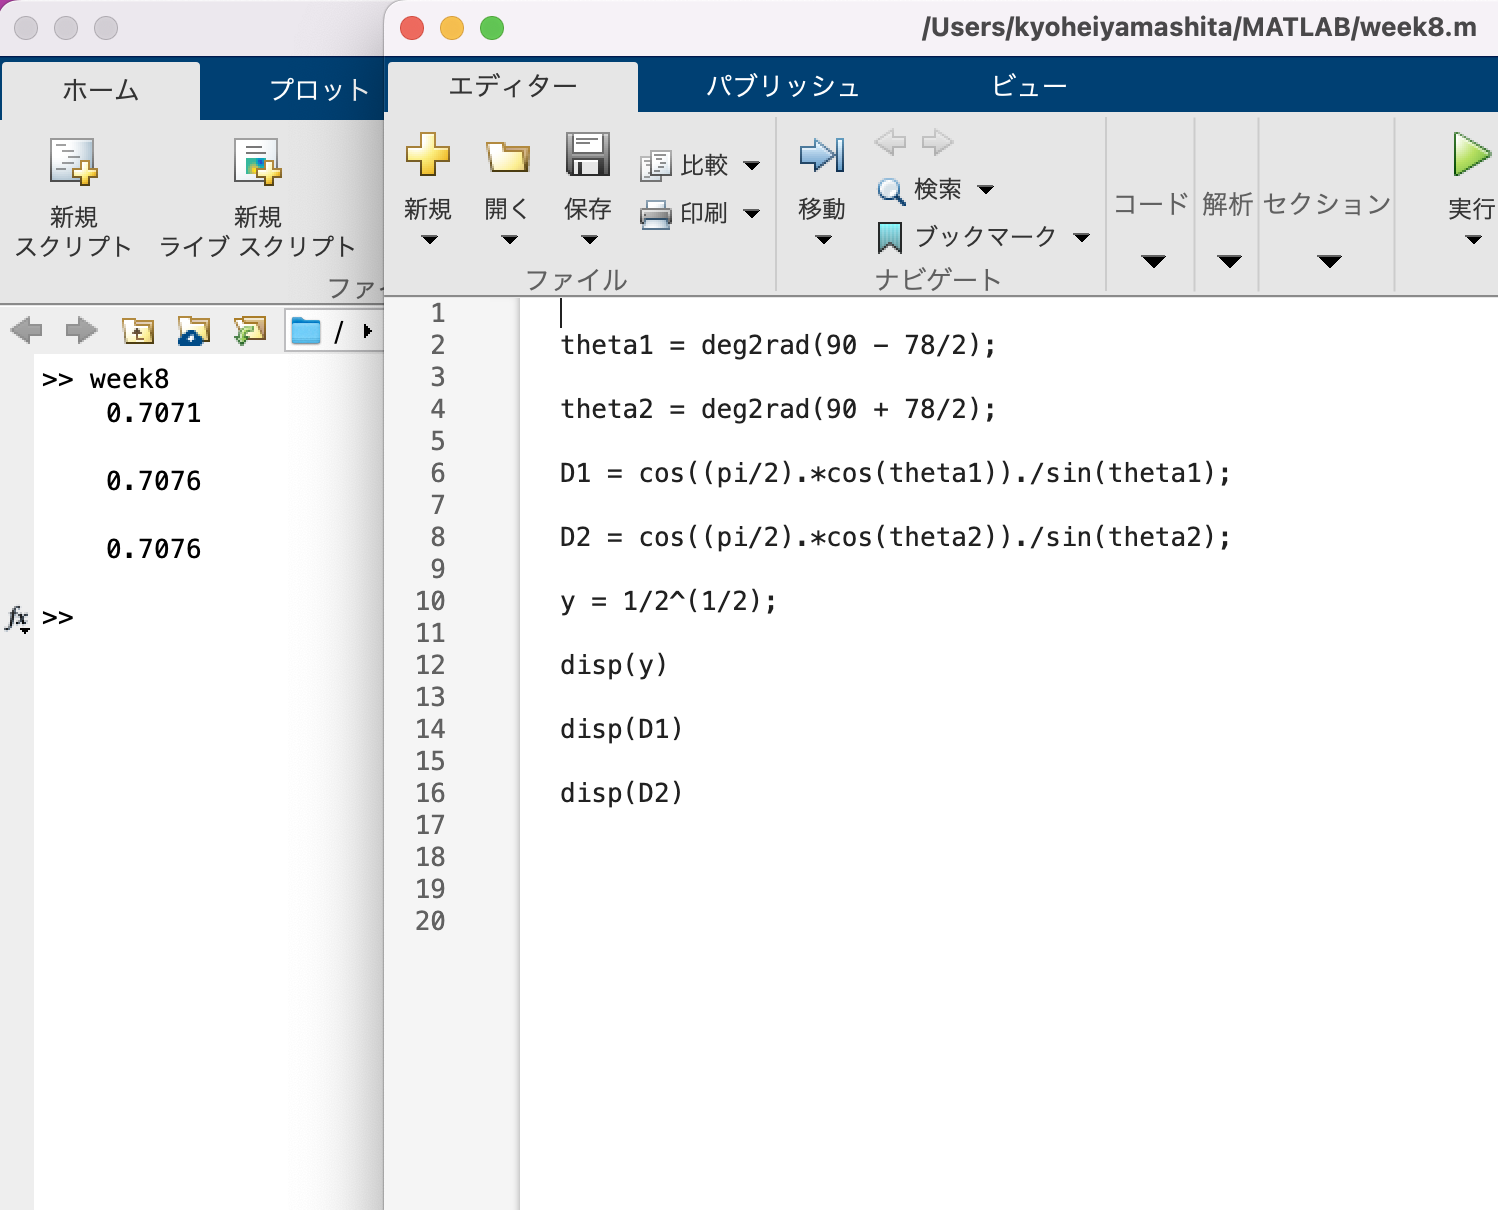
\includegraphics[scale=0.35]{pic1.png}
\end{figure}

出力結果より、値がほとんど\begin{math}\frac{1}{\sqrt{2}}\end{math}と一致していることが
確認できたので、半値角は78°である。

\section{評論}

大きさを半波長ほどに大きくした時、指向性をほとんど絞ることができない。
つまりは、大きくする必要性がほとんどないと考えられるので、微笑ダイポールアンテナ
は、大きさを考えた時実用的であるといえる。


\end{document}

